\documentclass[12pt]{article}
\usepackage{amsmath}
\usepackage{amssymb}
\usepackage{framed}
\usepackage{graphicx}
%opening

\begin{document}
\tableofcontents
\newpage
\section{Binomial Logistic Regression}
Binomial logistic regression estimates the probability of an event (as an example, having heart disease) occurring. 
\begin{itemize}
\item If the estimated probability of the event occurring is greater than or equal to 0.5 (better than even chance), the procedure classifies the event as occurring (e.g., heart disease being present). \item If the probability is less than 0.5, Logistic regression classifies the event as not occurring (e.g., no heart disease). 
\end{itemize}
\subsection{Category Prediction Table}




It is very common to use binomial logistic regression to predict whether cases can be correctly classified (i.e., predicted) from the independent variables. Therefore, it becomes necessary to have a method to assess the effectiveness of the predicted classification against the actual classification. There are many methods to assess this with their usefulness oftening depending on the nature of the study conducted. However, all methods revolve around the observed and predicted classifications, which are presented in the ``Classification Table", as shown below:

\begin{figure}[h!]
\centering
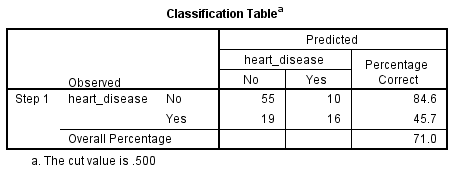
\includegraphics[width=0.97\linewidth]{BLogReg-Table}
\caption{SPSS Output}
\label{fig:BLogReg-Table}
\end{figure}

Firstly, notice that the table has a subscript which states, ``The cut value is .500". This means that if the probability of a case being classified into the "yes" category is greater than .500, then that particular case is classified into the "yes" category. 
Otherwise, the case is classified as in the "no" category. 

\subsection{Interpreting the Classifcation Table}
Whilst the classification table appears to be very simple, it actually provides a lot of important information about your binomial logistic regression result, including:

\begin{itemize}
\item[A.] The \textbf{percentage accuracy in classification (PAC)}, which reflects the percentage of cases that can be correctly classified as "no" heart disease with the independent variables added (not just the overall model).
\item[B.] \textbf{Sensitivity}, which is the percentage of cases that had the observed characteristic (e.g., "yes" for heart disease) which were correctly predicted by the model (i.e., true positives).
\item[C.] \textbf{Specificity}, which is the percentage of cases that did not have the observed characteristic (e.g., "no" for heart disease) and were also correctly predicted as not having the observed characteristic (i.e., true negatives).
\item[D.] The \textbf{positive predictive value}, which is the percentage of correctly predicted cases "with" the observed characteristic compared to the total number of cases predicted as having the characteristic.
\item[E.] The \textbf{negative predictive value}, which is the percentage of correctly predicted cases ``without" the observed characteristic compared to the total number of cases predicted as not having the characteristic.
\end{itemize}
\end{document}
